\input{defs}
\section{Experiments}

\subsection{Experimental Setup}

\noindent\textbf{Benchmark.}
We evaluate on \tbench~\citep{barres2025tau2benchevaluatingconversationalagents}, a multi-turn customer-service benchmark for tool-using LLM agents. We consider its two standard domains: \textsc{Airline}, which contains 50 tasks involving flight booking, modification, cancellation, and policy-sensitive customer requests, and \textsc{Retail}, which contains 114 tasks involving order management, exchanges, returns, and account updates. In both domains, the agent interacts with a simulated user over multiple turns and must complete the task by issuing tool calls in the environment.

Each task is evaluated using the benchmark's binary success criterion. A task is counted as solved only if the agent both executes the correct tool actions and communicates the required information to the user. Following the benchmark protocol, we report \emph{pass rate}, i.e., the fraction of tasks solved successfully.

\noindent\textbf{Evaluation protocol.}
Unless otherwise specified, we evaluate all models with greedy decoding (temperature $0.0$) to enable deterministic comparison between different models and techniques, a maximum context length of 32{,}000 tokens, and a maximum of 50 interaction steps per episode. We use a single evaluation trial per benchmark instance. The user simulator is the same base model as the evaluated agent.

\noindent\textbf{Base model.}
We use Qwen3-30B-A3B-Instruct-2507 as the base agent in all experiments. The model provides native tool-calling support and serves as the initialization for both our capability-specific training procedure and all comparison baselines.

\noindent\textbf{Training setup.}
Our method first identifies missing capabilities from failures in the target environment, synthesizes one micro-environment for each retained capability, and then trains a separate LoRA adapter for each capability using capability-specific reinforcement learning. Each adapter is trained with GRPO while keeping the base model frozen. Unless otherwise stated, we use LoRA rank $r=16$ and apply adapters to \texttt{q\_proj}, \texttt{k\_proj}, \texttt{v\_proj}, \texttt{o\_proj}, \texttt{gate\_proj}, \texttt{up\_proj}, and \texttt{down\_proj}. We optimize with AdamW at a learning rate of $10^{-5}$, use sampling temperature $1.0$ during rollout collection, and train each adapter independently for 10--40 iterations depending on the capability. GRPO is run without KL regularization. Training uses gradient checkpointing and distributed data parallelism on 4--8 A100-80GB GPUs. More training details are in Appendix. 

\noindent\textbf{Baselines.}
We compare against several categories of baselines in addition to the \emph{Base model} (Qwen3-30B-A3B-Instruct-2507) itself. 

First, we compare against recent approaches that use large-scale general-purpose synthetic data and environments to train agents. \emph{Agent World Model (AWM)} performs reinforcement learning in benchmark-independent synthetic environments that are procedurally generated to support broad tool-use training. Unlike our method, these environments are not constructed to isolate specific missing capabilities. \emph{Agent Data Protocol (ADP)}~\citep{song2026agentdataprotocol} performs supervised fine-tuning on diverse public agent trajectories unified under a common representation. These two baselines test whether large-scale general synthetic training can match the gains of our targeted, capability-specific framework.

Second, to demonstrate the need for training, we compare against a \emph{Prompting} baseline that augments the agent's system prompt with explicit descriptions of the capabilities it should exercise, without any additional training. Third, \emph{Single capability trained model} trains a single LoRA adapter on one synthesized capability environment, testing the effectiveness of the corresponding capability-targeted environment in isolation.

Finally, to highlight the challenge of consolidating all capabilities into a single model and motivate our routing approach, we implement and ablate several multi-capability methods. \emph{CORE-TSV merge} combines independently trained capability-specific adapters into a single model in a shared low-rank merging space following Core Space merging~\citep{panariello2025corespace}; the merge rule uses task-vector-style composition~\citep{ilharco2023taskarithmetic} with TIES-inspired sign resolution~\citep{yadav2023tiesmerging}. \emph{Mixed-environment GRPO} trains a single LoRA adapter on a uniform mixture of all synthesized capability environments, testing whether monolithic training on combined environments can lead to collective acquisition of all capabilities. \emph{SFT Synthetic} trains a single LoRA adapter on successful trajectories collected from all the synthesized capability environments. \emph{On-Policy Distillation} first trains a separate LoRA teacher adapter on each synthesized capability environment, then trains a single student LoRA on a uniform mixture of all environments: the student generates on-policy rollouts, and each rollout is scored by the corresponding capability-specific teacher that drives the student's token-level distributions toward each teacher's. We run each of these multicapability training approaches for the same number of training steps as training each capability separately. More details about these methods are provided in the Appendix.




\noindent\textbf{Metrics.}
We use pass rate as the primary evaluation metric, following the $\tau$-Bench protocol. A task is counted as solved only if it satisfies the benchmark's binary success criterion, which requires both correct task execution and correct communication with the user. We report pass rate separately for the \textsc{Airline} and \textsc{Retail} domains. When reporting an overall score, we compute the fraction of solved tasks over the union of both domains:

\[
\mathrm{PassRate}_{\mathrm{overall}}
=
\frac{\#_{\mathrm{Correct}\_{\mathrm{Airline}}} + \#_{\mathrm{Correct}\_{\mathrm{Retail}}}}{\#_{\mathrm{Airline}} + \#_{\mathrm{Retail}}}.
\]


\input{tables/main_res}

\subsection{Effectiveness of Method}

Table~\ref{tab:main_tb_results} summarizes results. Our full method (Routing) achieves 45.1\% overall, improving over the base model by +12.2 points and over the strongest external baseline (AWM) by +6.7 points.

\noindent\textbf{Capability-targeted training outperforms general-purpose training in accuracy and efficiency.}
Even a single adapter trained on one synthesized capability environment (40.3\%) surpasses both AWM (38.4\%), which trains on diverse procedurally generated environments, and ADP (32.3\%), which fine-tunes on diverse public agent trajectories. ADP actually \emph{degrades} Retail performance relative to the base model (34.2\% vs.\ 36.8\%), indicating that general-purpose trajectory data can harm environment-specific performance. This gap is especially striking given the scale disparity: AWM synthesizes over 1{,}000 code-driven agentic environments, while our full method uses only four capability-specific ones, yet a single targeted adapter already outperforms it (+1.9 overall). Precisely diagnosing missing capabilities and training on targeted environments is far more data-efficient than scaling the breadth of synthetic training.

\noindent\textbf{Routing outperforms all methods that consolidate capabilities into one model.}
A single adapter cannot cover the benchmark's diverse capabilities. Routing exceeds the best single adapter by +4.8 points (45.1\% vs.\ 40.3\%) and every consolidation method: CORE-TSV merge (39.6\%), On-Policy Distillation (37.8\%), SFT Synthetic (37.8\%), and Mixed-environment GRPO (40.9\%). In On-Policy Distillation, each teacher's distributions are shaped by its synthetic environment; the student must match all teachers simultaneously and ends up failing to reach the performance of any. Similarly, in SFT Synthetic, the model imitates successful trajectories but cannot disentangle transferable capabilities from trajectories of each synthetic environment, so the learned behaviors compose poorly. Mixed GRPO similarly cannot escape gradient interference when all capabilities share the same adapter weights. 

\noindent\textbf{Training is essential---capability identification alone is insufficient.}
Prompting the base model with capability descriptions (37.2\%) outperforms both ADP and the base model, confirming that capability identification has independent value. However, Routing surpasses Prompting by +7.9 points, with the gap widening on Retail (47.4\% vs.\ 38.6\%): \emph{knowing which capabilities to exercise} is not a substitute for \emph{learning to exercise them}. These findings collectively demonstrate that the full pipeline---identify, synthesize, train, and route---is necessary to realize the method's full potential.






% \subsection{Analysis of Synthesized Envs}
\subsection{Analysis of Synthesized Environments}

Our synthesized micro-environments preserve the target benchmark's tool interface and policy constraints while procedurally generating novel task instances that isolate recurring capability deficits. The retained environments target failures in structured data reasoning, multi-step task completion, precondition verification, tool-calling precision, and adversarial policy compliance. This yields training environments that remain aligned with the target environment at the level of actions and verification, while avoiding direct training on benchmark tasks.

Across all retained capabilities, the synthesized environments satisfy three common design principles. They are \emph{interface-faithful}, in that they use the same tool schemas and state representation as the target benchmark; \emph{capability-isolating}, in that success depends primarily on one missing behavior; and \emph{verifiable}, in that reward can be computed automatically from tool arguments, or policy-consistent outcomes. Although each environment is designed to isolate a dominant failure mode, the capabilities are not assumed to be strictly disjoint: a single failed benchmark trajectory may reflect multiple deficits, and therefore may be covered by more than one synthesized environment.



\begin{figure*}[t]
    \centering
    \begin{subfigure}[t]{0.48\textwidth}
        \centering
        
\includegraphics[width=\textwidth]{figures/plot_selection_frequency.png}
        \caption{Capability selection frequency across 10 independent analysis runs by the analysis agent.}
        \label{fig:capability_selection}
    \end{subfigure}
    \hfill
    \begin{subfigure}[t]{0.48\textwidth}
        \centering
        
\includegraphics[width=\textwidth]{figures/plot_skill_coverage.png}
        \caption{Capability coverage over failed benchmark tasks. Bars show the median number of covered failures across runs; error bars denote the interquartile range. Coverage is not mutually exclusive across capabilities.}
        \label{fig:capability_coverage}
    \end{subfigure}
    \caption{Stability and coverage of the capabilities used to synthesize micro-environments. Repeated contrastive analysis of target-environment failures identifies a small set of high-impact, recurring capability deficits.}
    \label{fig:capability_analysis}
\end{figure*}

Figure~\ref{fig:capability_analysis} summarizes the capabilities identified by repeated contrastive analysis of target-environment failures. Figure~\ref{fig:capability_analysis}(a) shows the selection frequency of each candidate capability across 10 independent analysis runs. Three capabilities: structured data reasoning, multi-step task completion, and precondition verification, are selected in all 10 runs, while tool-calling precision is selected in 8 of 10 runs. Adversarial policy compliance is selected less consistently, appearing in 4 of 10 runs, suggesting that it captures a real but more context-dependent failure mode. In contrast, competing capability categories such as conditional reasoning, numerical reasoning, early termination, and information communication are selected much less frequently. This indicates that the synthesized environments are not chosen arbitrarily, but instead correspond to stable and recurring capability deficits exposed by the benchmark.

Figure~\ref{fig:capability_analysis}(b) shows the median failure coverage of each capability, with error bars denoting the interquartile range across analysis runs. Structured data reasoning covers the largest portion of failed tasks, followed by multi-step task completion and tool-calling precision, while precondition verification and adversarial policy compliance cover smaller but still recurring subsets of failures. Because a single failed benchmark trajectory may involve multiple missing capabilities, these coverage counts are not mutually exclusive. Taken together, the selection-frequency and coverage results support our environment design: a small set of synthesized environments captures the dominant and consistently recurring capability gaps in the target environment, allowing training to focus on the behaviors most responsible for benchmark failures.

Two patterns emerge from this analysis. First, the selected environment set is stable across repeated runs of the analysis procedure. Three environments are recovered in all 10 runs, and tool calling precision is recovered in 8 of 10 runs, indicating substantial overlap among independently generated diagnoses. The only less stable environment is adversarial policy compliance, which appears in 4 of 10 runs; this suggests that the corresponding failure mode is real but less prevalent and more context-dependent than the other deficits.

Second, failure coverage is concentrated in a small number of environments. Structured data reasoning has the highest median coverage, followed by multi-step task completion and tool calling precision, indicating that these deficits account for a substantial fraction of observed failures. Precondition verification and adversarial policy compliance cover smaller but still recurring subsets of failures. This concentration supports our decision to synthesize a small number of targeted environments rather than optimize over a broad and undifferentiated mixture of tasks.

Overall, these results suggest that the synthesized environments capture recurring, high-impact capability deficits exposed by the target benchmark, while remaining stable enough across repeated analyses to support automated environment generation. They also provide a concrete explanation for where the training signal is concentrated: rather than distributing optimization uniformly across all behaviors, the framework focuses on the environments that cover the largest and most consistently observed failure modes.


\subsection{Method Scaling}

\begin{figure*}[t]
    \centering
    \begin{subfigure}[t]{0.48\textwidth}
        \centering
        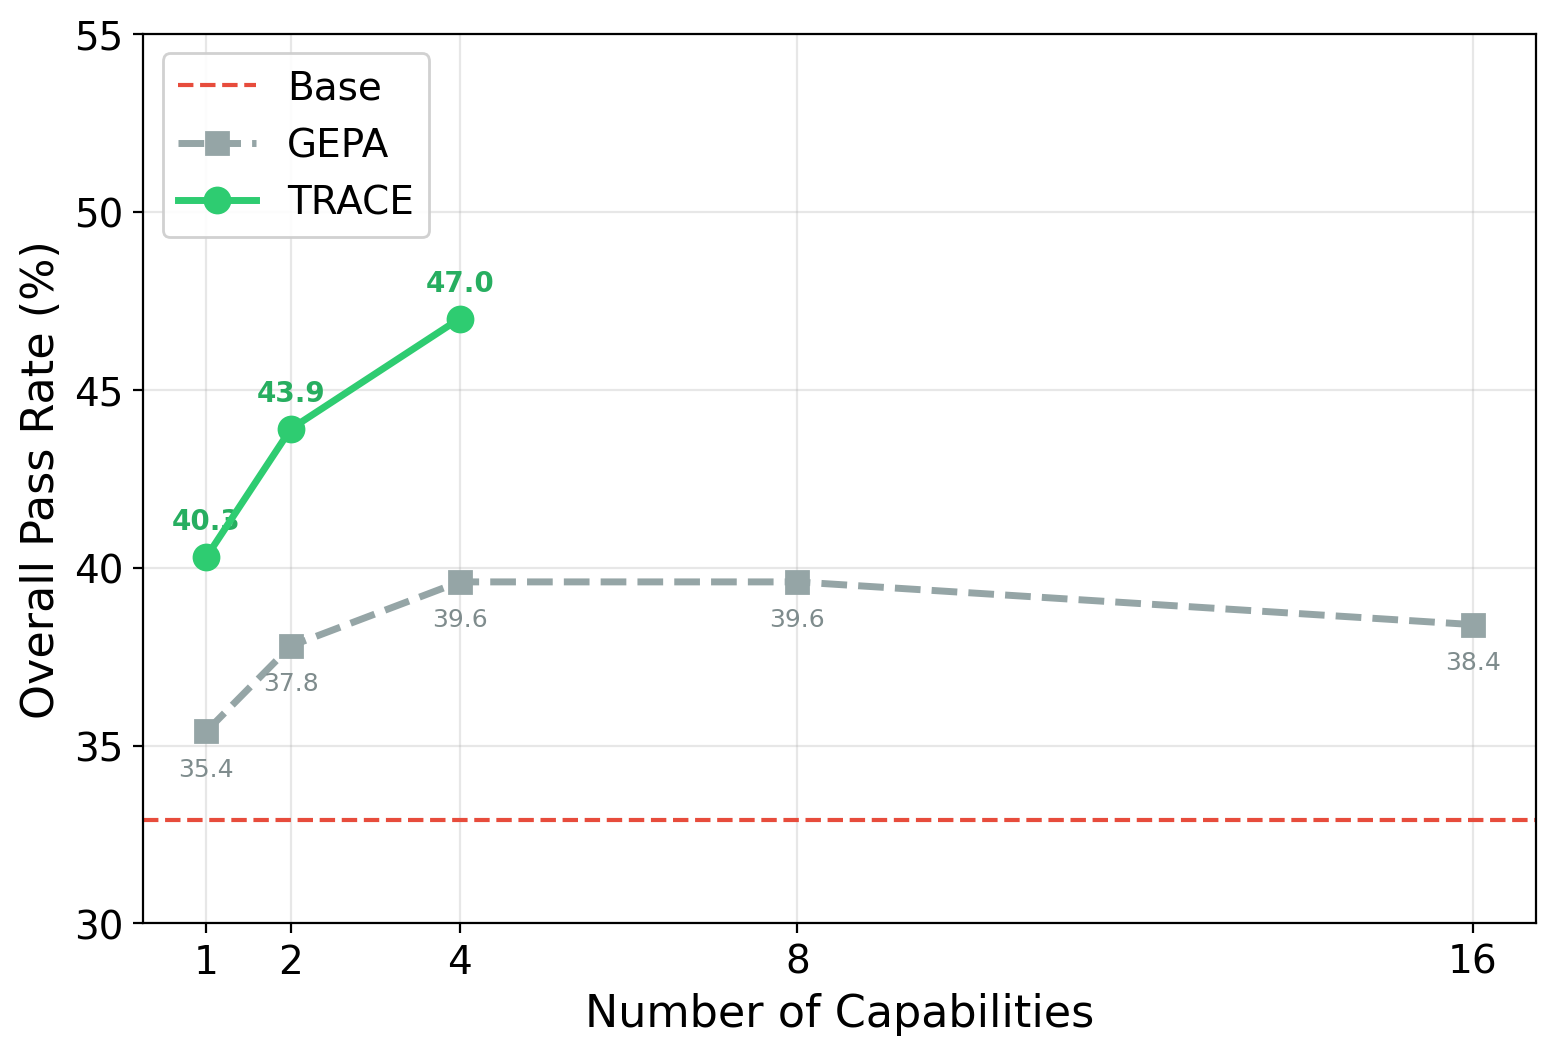
\includegraphics[width=\textwidth]{figures/cap_scaling.png}
        \caption{Performance scaling with the number of capabilities. Routing outperforms injecting capabilities descriptions into the prompt, which peaks and degrades as more are added in context.}
        \label{fig:cap_scaling}
    \end{subfigure}
    \hfill
    \begin{subfigure}[t]{0.48\textwidth}
        \centering
        % TODO: add right subfigure
        \label{fig:cap_scaling_right}
    \end{subfigure}
    \caption{Scaling behavior of our method.}
    \label{fig:scaling}
\end{figure*}

\paragraph{Scaling the number of capabilities}
Figure~\ref{fig:cap_scaling} shows how performance scales with the number of capabilities. Prompting with capability descriptions peaks at 38.4\% with four descriptions (failing to reach the performance of training on even one capability) and then degrades to 35.1\% with sixteen as additional descriptions dilute the context. These results show that prompting even with a larger number of capabilities is insufficient to reach the performance that training confers.



\paragraph{Scaling the number of training steps}

show scaling the number of training steps on 1 skill targeted synthetic env outperforms direct Rl on the env with same number of steps
